\documentclass[11pt,compress,t,notes=noshow, xcolor=table]{beamer}
% graphicx and color are loaded via lmu-lecture.sty
% maxwidth is the original width if it is less than linewidth
% otherwise use linewidth (to make sure the graphics do not exceed the margin)
% TODO: Remove once cleared to be superfluous
% \makeatletter
% \def\maxwidth{ %
%   \ifdim\Gin@nat@width>\linewidth
%     \linewidth
%   \else
%     \Gin@nat@width
%   \fi
% }
% \makeatother

% ---------------------------------%
% latex-math dependencies, do not remove:
% - mathtools
% - bm
% - siunitx
% - dsfont
% - xspace
% ---------------------------------%

%--------------------------------------------------------%
%       Language, encoding, typography
%--------------------------------------------------------%

\usepackage[english]{babel}
\usepackage[utf8]{inputenc} % Enables inputting UTF-8 symbols
% Standard AMS suite (loaded via lmu-lecture.sty)

% Font for double-stroke / blackboard letters for sets of numbers (N, R, ...)
% Distribution name is "doublestroke"
% According to https://mirror.physik.tu-berlin.de/pub/CTAN/fonts/doublestroke/dsdoc.pdf
% the "bbm" package does a similar thing and may be superfluous.
% Required for latex-math
\usepackage{dsfont}

% bbm – "Blackboard-style" cm fonts (https://www.ctan.org/pkg/bbm)
% Used to be in common.tex, loaded directly after this file
% Maybe superfluous given dsfont is loaded
% TODO: Check if really unused?
% \usepackage{bbm}

% bm – Access bold symbols in maths mode - https://ctan.org/pkg/bm
% Required for latex-math, preferred over \boldsymbol
% https://tex.stackexchange.com/questions/3238/bm-package-versus-boldsymbol
\usepackage{bm}

% pifont – Access to PostScript standard Symbol and Dingbats fonts
% Used for \newcommand{\xmark}{\ding{55}, which is never used
% aside from lecture_advml/attic/xx-automl/slides.Rnw
% \usepackage{pifont}

% Quotes (inline and display), provdes \enquote
% https://ctan.org/pkg/csquotes
\usepackage{csquotes}

% Adds arg to enumerate env, technically superseded by enumitem according
% to https://ctan.org/pkg/enumerate
% Replace with https://ctan.org/pkg/enumitem ?
% Even better: enumitem is not really compatible with beamer and breaks all sorts of things
% particularly the enumerate environment. The enumerate package also just isn't required
% from what I can tell so... don't re-add it I guess?
% \usepackage{enumerate}

% Line spacing - provides \singlespacing \doublespacing \onehalfspacing
% https://ctan.org/pkg/setspace
% \usepackage{setspace}

% mathtools – Mathematical tools to use with amsmath
% https://ctan.org/pkg/mathtools?lang=en
% latex-math dependency according to latex-math repo
\usepackage{mathtools}

% Maybe not great to use this https://tex.stackexchange.com/a/197/19093
% Use align instead -- TODO: Global search & replace to check, eqnarray is used a lot
% $ rg -f -u "\begin{eqnarray" -l | grep -v attic | awk -F '/' '{print $1}' | sort | uniq -c
%   13 lecture_advml
%   14 lecture_i2ml
%    2 lecture_iml
%   27 lecture_optimization
%   45 lecture_sl
\usepackage{eqnarray}
% For shaded regions / boxes
% Used sometimes in optim
% https://www.ctan.org/pkg/framed
\usepackage{framed}

%--------------------------------------------------------%
%       Cite button (version 2024-05)
%--------------------------------------------------------%

% Superseded by style/ref-buttons.sty, kept just in case these don't work out somehow.

% Note this requires biber to be in $PATH when running,
% telltale error in log would be e.g. Package biblatex Info: ... file 'authoryear.dbx' not found
% aside from obvious "biber: command not found" or similar.
% Tried moving this to lmu-lecture.sty but had issues I didn't quite understood,
% so it's here for now.

\usepackage{hyperref}

% Only try adding a references file if it exists, otherwise
% this would compile error when references.bib is not found
% NOTE: Bibliography packages (usebib, biblatex) are now loaded by ref-buttons.sty when needed
% This keeps all bibliography-related setup in one place

% Legacy \citelink command removed - superseded by ref-buttons.sty

%--------------------------------------------------------%
%       Displaying code and algorithms
%--------------------------------------------------------%

% Reimplements verbatim environments: https://ctan.org/pkg/verbatim
% verbatim used sed at least once in
% supervised-classification/slides-classification-tasks.tex
% Removed since code should not be put on slides anyway
% \usepackage{verbatim}

% Both used together for algorithm typesetting, see also overleaf: https://www.overleaf.com/learn/latex/Algorithms
% algorithmic env is also used, but part of the bundle:
%   "algpseudocode is part of the algorithmicx bundle, it gives you an improved version of algorithmic besides providing some other features"
% According to https://tex.stackexchange.com/questions/229355/algorithm-algorithmic-algorithmicx-algorithm2e-algpseudocode-confused
\usepackage{algorithm}
\usepackage{algpseudocode}

%--------------------------------------------------------%
%       Tables
%--------------------------------------------------------%

% multi-row table cells: https://www.namsu.de/Extra/pakete/Multirow.html
% Provides \multirow
% Used e.g. in evaluation/slides-evaluation-measures-classification.tex
\usepackage{multirow}

% colortbl: https://ctan.org/pkg/colortbl
% "The package allows rows and columns to be coloured, and even individual cells." well.
% Provides \columncolor and \rowcolor
% \rowcolor is used multiple times, e.g. in knn/slides-knn.tex
\usepackage{colortbl}

% long/multi-page tables: https://texdoc.org/serve/longtable.pdf/0
% Not used in slides
% \usepackage{longtable}

% pretty table env: https://ctan.org/pkg/booktabs
% Is used
% Defines \toprule
\usepackage{booktabs}

%--------------------------------------------------------%
%       Figures: Creating, placing, verbing
%--------------------------------------------------------%

% wrapfig - Wrapping text around figures https://de.overleaf.com/learn/latex/Wrapping_text_around_figures
% Provides wrapfigure environment -used in lecture_optimization
\usepackage{wrapfig}

% Sub figures in figures and tables
% https://ctan.org/pkg/subfig -- supersedes subfigure package
% Provides \subfigure
% \subfigure not used in slides but slides-tuning-practical.pdf errors without this pkg, error due to \captionsetup undefined
\usepackage{subfig}

% Actually it's pronounced PGF https://en.wikibooks.org/wiki/LaTeX/PGF/TikZ
\usepackage{tikz}

% No idea what/why these settings are what they are but I assume they're there on purpose
\usetikzlibrary{shapes,arrows,automata,positioning,calc,chains,trees, shadows}
\tikzset{
  %Define standard arrow tip
  >=stealth',
  %Define style for boxes
  punkt/.style={
    rectangle,
    rounded corners,
    draw=black, very thick,
    text width=6.5em,
    minimum height=2em,
    text centered},
  % Define arrow style
  pil/.style={
    ->,
    thick,
    shorten <=2pt,
    shorten >=2pt,}
}

%--------------------------------------------------------%
%       Beamer setup and custom macros & environments
%--------------------------------------------------------%

% Main sty file for beamer setup (layout, style, lecture page numbering, etc.)
% For long-term maintenance, this may me refactored into a more modular set of .sty files
\usepackage{../../style/lmu-lecture}
% Custom itemize wrappers, itemizeS, itemizeL, etc
\usepackage{../../style/customitemize}
% Custom framei environment, uses custom itemize!
\usepackage{../../style/framei}
% Custom frame2 environment, allows specifying font size for all content
\usepackage{../../style/frame2}
% Column layout macros
\usepackage{../../style/splitV}
% \image and derivatives
\usepackage{../../style/image}
% New generation of reference button macros
\usepackage{../../style/ref-buttons}

% Used regularly
\let\code=\texttt

% Not sure what/why this does
\setkeys{Gin}{width=0.9\textwidth}

% -- knitr leftovers --
% These may be used by knitr/R Markdown workflows in other lectures
\makeatletter
\def\maxwidth{ %
  \ifdim\Gin@nat@width>\linewidth
    \linewidth
  \else
    \Gin@nat@width
  \fi
}
\makeatother

% Define colors for syntax highlighting (may be used by knitr)
\definecolor{fgcolor}{rgb}{0.345, 0.345, 0.345}
\definecolor{shadecolor}{rgb}{.97, .97, .97}

% knitr code output environment
\newenvironment{knitrout}{}{}


% Can't find a reason why common.tex is not just part of this file?
\input{../../style/common}

\input{../../latex-math/basic-math}
% machine learning
\newcommand{\Xspace}{\mathcal{X}} % X, input space
\newcommand{\Yspace}{\mathcal{Y}} % Y, output space
\newcommand{\Zspace}{\mathcal{Z}} % Z, space of sampled datapoints
\newcommand{\nset}{\{1, \ldots, n\}} % set from 1 to n
\newcommand{\pset}{\{1, \ldots, p\}} % set from 1 to p
\newcommand{\gset}{\{1, \ldots, g\}} % set from 1 to g
\newcommand{\Pxy}{\mathbb{P}_{xy}} % P_xy
\newcommand{\Exy}{\mathbb{E}_{xy}} % E_xy: Expectation over random variables xy
\newcommand{\xv}{\mathbf{x}} % vector x (bold)
\newcommand{\xtil}{\tilde{\mathbf{x}}} % vector x-tilde (bold)
\newcommand{\yv}{\mathbf{y}} % vector y (bold)
\newcommand{\xy}{(\xv, y)} % observation (x, y)
\newcommand{\xvec}{\left(x_1, \ldots, x_p\right)^\top} % (x1, ..., xp)
\newcommand{\Xmat}{\mathbf{X}} % Design matrix
\newcommand{\allDatasets}{\mathds{D}} % The set of all datasets
\newcommand{\allDatasetsn}{\mathds{D}_n}  % The set of all datasets of size n
\newcommand{\D}{\mathcal{D}} % D, data
\newcommand{\Dn}{\D_n} % D_n, data of size n
\newcommand{\Dtrain}{\mathcal{D}_{\text{train}}} % D_train, training set
\newcommand{\Dtest}{\mathcal{D}_{\text{test}}} % D_test, test set
\newcommand{\xyi}[1][i]{\left(\xv^{(#1)}, y^{(#1)}\right)} % (x^i, y^i), i-th observation
\newcommand{\Dset}{\left( \xyi[1], \ldots, \xyi[n]\right)} % {(x1,y1)), ..., (xn,yn)}, data
\newcommand{\defAllDatasetsn}{(\Xspace \times \Yspace)^n} % Def. of the set of all datasets of size n
\newcommand{\defAllDatasets}{\bigcup_{n \in \N}(\Xspace \times \Yspace)^n} % Def. of the set of all datasets
\newcommand{\xdat}{\left\{ \xv^{(1)}, \ldots, \xv^{(n)}\right\}} % {x1, ..., xn}, input data
\newcommand{\ydat}{\left\{ \yv^{(1)}, \ldots, \yv^{(n)}\right\}} % {y1, ..., yn}, input data
\newcommand{\yvec}{\left(y^{(1)}, \hdots, y^{(n)}\right)^\top} % (y1, ..., yn), vector of outcomes
\newcommand{\greekxi}{\xi} % Greek letter xi
\renewcommand{\xi}[1][i]{\xv^{(#1)}} % x^i, i-th observed value of x
\newcommand{\yi}[1][i]{y^{(#1)}} % y^i, i-th observed value of y
\newcommand{\xivec}{\left(x^{(i)}_1, \ldots, x^{(i)}_p\right)^\top} % (x1^i, ..., xp^i), i-th observation vector
\newcommand{\xj}{\xv_j} % x_j, j-th feature
\newcommand{\xjvec}{\left(x^{(1)}_j, \ldots, x^{(n)}_j\right)^\top} % (x^1_j, ..., x^n_j), j-th feature vector
\newcommand{\phiv}{\mathbf{\phi}} % Basis transformation function phi
\newcommand{\phixi}{\mathbf{\phi}^{(i)}} % Basis transformation of xi: phi^i := phi(xi)

%%%%%% ml - models general
\newcommand{\lamv}{\bm{\lambda}} % lambda vector, hyperconfiguration vector
\newcommand{\Lam}{\Lambda}	 % Lambda, space of all hpos
% Inducer / Inducing algorithm
\newcommand{\preimageInducer}{\left(\defAllDatasets\right)\times\Lam} % Set of all datasets times the hyperparameter space
\newcommand{\preimageInducerShort}{\allDatasets\times\Lam} % Set of all datasets times the hyperparameter space
% Inducer / Inducing algorithm
\newcommand{\ind}{\mathcal{I}} % Inducer, inducing algorithm, learning algorithm

% continuous prediction function f
\newcommand{\ftrue}{f_{\text{true}}}  % True underlying function (if a statistical model is assumed)
\newcommand{\ftruex}{\ftrue(\xv)} % True underlying function (if a statistical model is assumed)
\newcommand{\fx}{f(\xv)} % f(x), continuous prediction function
\newcommand{\fdomains}{f: \Xspace \rightarrow \R^g} % f with domain and co-domain
\newcommand{\Hspace}{\mathcal{H}} % hypothesis space where f is from
\newcommand{\Hall}{\mathcal{H}_{\text{all}}} % unrestricted hypothesis space
\newcommand{\fbayes}{f^{\ast}} % Bayes-optimal model
\newcommand{\fxbayes}{f^{\ast}(\xv)} % Bayes-optimal model
\newcommand{\fkx}[1][k]{f_{#1}(\xv)} % f_j(x), discriminant component function
\newcommand{\fhspace}{\hat f_{\Hspace}} % fhat_H
\newcommand{\fh}{\hat{f}} % f hat, estimated prediction function
\newcommand{\fxh}{\fh(\xv)} % fhat(x)
\newcommand{\fxt}{f(\xv ~|~ \thetav)} % f(x | theta)
\newcommand{\fxi}{f\left(\xv^{(i)}\right)} % f(x^(i))
\newcommand{\fxih}{\hat{f}\left(\xv^{(i)}\right)} % f(x^(i))
\newcommand{\fxit}{f\big(\xv^{(i)} ~|~ \thetav\big)} % f(x^(i) | theta)
\newcommand{\fhD}{\fh_{\D}} % fhat_D, estimate of f based on D
\newcommand{\fhDtrain}{\fh_{\Dtrain}} % fhat_Dtrain, estimate of f based on D
\newcommand{\fhDnlam}{\fh_{\Dn, \lamv}} %model learned on Dn with hp lambda
\newcommand{\fhDlam}{\fh_{\D, \lamv}} %model learned on D with hp lambda
\newcommand{\fhDnlams}{\fh_{\Dn, \lamv^\ast}} %model learned on Dn with optimal hp lambda
\newcommand{\fhDlams}{\fh_{\D, \lamv^\ast}} %model learned on D with optimal hp lambda

% discrete prediction function h
\newcommand{\hx}{h(\xv)} % h(x), discrete prediction function
\newcommand{\hh}{\hat{h}} % h hat
\newcommand{\hxh}{\hat{h}(\xv)} % hhat(x)
\newcommand{\hxt}{h(\xv | \thetav)} % h(x | theta)
\newcommand{\hxi}{h\left(\xi\right)} % h(x^(i))
\newcommand{\hxit}{h\left(\xi ~|~ \thetav\right)} % h(x^(i) | theta)
\newcommand{\hbayes}{h^{\ast}} % Bayes-optimal classification model
\newcommand{\hxbayes}{h^{\ast}(\xv)} % Bayes-optimal classification model

% yhat
\newcommand{\yh}{\hat{y}} % yhat for prediction of target
\newcommand{\yih}{\hat{y}^{(i)}} % yhat^(i) for prediction of ith targiet
\newcommand{\resi}{\yi- \yih}

% theta
\newcommand{\thetah}{\hat{\theta}} % theta hat
\newcommand{\thetav}{\bm{\theta}} % theta vector
\newcommand{\thetavh}{\bm{\hat\theta}} % theta vector hat
\newcommand{\thetat}[1][t]{\thetav^{[#1]}} % theta^[t] in optimization
\newcommand{\thetatn}[1][t]{\thetav^{[#1 +1]}} % theta^[t+1] in optimization
\newcommand{\thetahDnlam}{\thetavh_{\Dn, \lamv}} %theta learned on Dn with hp lambda
\newcommand{\thetahDlam}{\thetavh_{\D, \lamv}} %theta learned on D with hp lambda
\newcommand{\mint}{\min_{\thetav \in \Theta}} % min problem theta
\newcommand{\argmint}{\argmin_{\thetav \in \Theta}} % argmin theta

% densities + probabilities
% pdf of x
\newcommand{\pdf}{p} % p
\newcommand{\pdfx}{p(\xv)} % p(x)
\newcommand{\pixt}{\pi(\xv~|~ \thetav)} % pi(x|theta), pdf of x given theta
\newcommand{\pixit}[1][i]{\pi\left(\xi[#1] ~|~ \thetav\right)} % pi(x^i|theta), pdf of x given theta
\newcommand{\pixii}[1][i]{\pi\left(\xi[#1]\right)} % pi(x^i), pdf of i-th x

% pdf of (x, y)
\newcommand{\pdfxy}{p(\xv,y)} % p(x, y)
\newcommand{\pdfxyt}{p(\xv, y ~|~ \thetav)} % p(x, y | theta)
\newcommand{\pdfxyit}{p\left(\xi, \yi ~|~ \thetav\right)} % p(x^(i), y^(i) | theta)

% pdf of x given y
\newcommand{\pdfxyk}[1][k]{p(\xv | y= #1)} % p(x | y = k)
\newcommand{\lpdfxyk}[1][k]{\log p(\xv | y= #1)} % log p(x | y = k)
\newcommand{\pdfxiyk}[1][k]{p\left(\xi | y= #1 \right)} % p(x^i | y = k)

% prior probabilities
\newcommand{\pik}[1][k]{\pi_{#1}} % pi_k, prior
\newcommand{\pih}{\hat{\pi}} % pi hat, estimated prior (binary classification)
\newcommand{\pikh}[1][k]{\hat{\pi}_{#1}} % pi_k hat, estimated prior
\newcommand{\lpik}[1][k]{\log \pi_{#1}} % log pi_k, log of the prior
\newcommand{\pit}{\pi(\thetav)} % Prior probability of parameter theta

% posterior probabilities
\newcommand{\post}{\P(y = 1 ~|~ \xv)} % P(y = 1 | x), post. prob for y=1
\newcommand{\postk}[1][k]{\P(y = #1 ~|~ \xv)} % P(y = k | y), post. prob for y=k
\newcommand{\pidomains}{\pi: \Xspace \rightarrow \unitint} % pi with domain and co-domain
\newcommand{\pibayes}{\pi^{\ast}} % Bayes-optimal classification model
\newcommand{\pixbayes}{\pi^{\ast}(\xv)} % Bayes-optimal classification model
\newcommand{\piastxtil}{\pi^{\ast}(\xtil)} % Bayes-optimal classification model
\newcommand{\piastkxtil}{\pi^{\ast}_k(\xtil)} % Bayes-optimal classification model for k-th class
\newcommand{\pix}{\pi(\xv)} % pi(x), P(y = 1 | x)
\newcommand{\piv}{\bm{\pi}} % pi, bold, as vector
\newcommand{\pikx}[1][k]{\pi_{#1}(\xv)} % pi_k(x), P(y = k | x)
\newcommand{\pikxt}[1][k]{\pi_{#1}(\xv ~|~ \thetav)} % pi_k(x | theta), P(y = k | x, theta)
\newcommand{\pixh}{\hat \pi(\xv)} % pi(x) hat, P(y = 1 | x) hat
\newcommand{\pikxh}[1][k]{\hat \pi_{#1}(\xv)} % pi_k(x) hat, P(y = k | x) hat
\newcommand{\pixih}{\hat \pi(\xi)} % pi(x^(i)) with hat
\newcommand{\pikxih}[1][k]{\hat \pi_{#1}(\xi)} % pi_k(x^(i)) with hat
\newcommand{\pdfygxt}{p(y ~|~\xv, \thetav)} % p(y | x, theta)
\newcommand{\pdfyigxit}{p\left(\yi ~|~\xi, \thetav\right)} % p(y^i |x^i, theta)
\newcommand{\lpdfygxt}{\log \pdfygxt } % log p(y | x, theta)
\newcommand{\lpdfyigxit}{\log \pdfyigxit} % log p(y^i |x^i, theta)

% probabilistic
\newcommand{\bayesrulek}[1][k]{\frac{\P(\xv | y= #1) \P(y= #1)}{\P(\xv)}} % Bayes rule
\newcommand{\muv}{\bm{\mu}} % expectation vector of Gaussian
\newcommand{\muk}[1][k]{\bm{\mu_{#1}}} % mean vector of class-k Gaussian (discr analysis)
\newcommand{\mukh}[1][k]{\bm{\hat{\mu}_{#1}}} % estimated mean vector of class-k Gaussian (discr analysis)

% residual and margin
\newcommand{\rx}{r(\xv)} % residual 
\newcommand{\eps}{\epsilon} % residual, stochastic
\newcommand{\epsv}{\bm{\epsilon}} % residual, stochastic, as vector
\newcommand{\epsi}{\epsilon^{(i)}} % epsilon^i, residual, stochastic
\newcommand{\epsh}{\hat{\epsilon}} % residual, estimated
\newcommand{\epsvh}{\hat{\epsv}} % residual, estimated, vector
\newcommand{\yf}{y \fx} % y f(x), margin
\newcommand{\yfi}{\yi \fxi} % y^i f(x^i), margin
\newcommand{\Sigmah}{\hat \Sigma} % estimated covariance matrix
\newcommand{\Sigmahj}{\hat \Sigma_j} % estimated covariance matrix for the j-th class
\newcommand{\nux}{\nu(\xv)} % nu(x) = y * f(x)

% ml - loss, risk, likelihood
\newcommand{\Lyf}{L\left(y, f\right)} % L(y, f), loss function
% \newcommand{\Lypi}{L\left(y, \pi\right)} % L(y, pi), loss function
\newcommand{\Lxy}{L\left(y, \fx\right)} % L(y, f(x)), loss function
\newcommand{\Lxyi}{L\left(\yi, \fxi\right)} % loss of observation
\newcommand{\Lxyt}{L\left(y, \fxt\right)} % loss with f parameterized
\newcommand{\Lxyit}{L\left(\yi, \fxit\right)} % loss of observation with f parameterized
\newcommand{\Lxym}{L\left(\yi, f\left(\bm{\tilde{x}}^{(i)} ~|~ \thetav\right)\right)} % loss of observation with f parameterized
\newcommand{\Lpixy}{L\left(y, \pix\right)} % loss in classification
% \newcommand{\Lpiy}{L\left(y, \pi\right)} % loss in classification
\newcommand{\Lpiv}{L\left(y, \piv\right)} % loss in classification
\newcommand{\Lpixyi}{L\left(\yi, \pixii\right)} % loss of observation in classification
\newcommand{\Lpixyt}{L\left(y, \pixt\right)} % loss with pi parameterized
\newcommand{\Lpixyit}{L\left(\yi, \pixit\right)} % loss of observation with pi parameterized
% \newcommand{\Lhy}{L\left(y, h\right)} % L(y, h), loss function on discrete classes
\newcommand{\Lhxy}{L\left(y, \hx\right)} % L(y, h(x)), loss function on discrete classes
\newcommand{\Lr}{L\left(r\right)} % L(r), loss defined on residual (reg) / margin (classif)
\newcommand{\lone}{|y - \fx|} % L1 loss
\newcommand{\ltwo}{\left(y - \fx\right)^2} % L2 loss
\newcommand{\lbernoullimp}{\ln(1 + \exp(-y \cdot \fx))} % Bernoulli loss for -1, +1 encoding
\newcommand{\lbernoullizo}{- y \cdot \fx + \log(1 + \exp(\fx))} % Bernoulli loss for 0, 1 encoding
\newcommand{\lcrossent}{- y \log \left(\pix\right) - (1 - y) \log \left(1 - \pix\right)} % cross-entropy loss
\newcommand{\lbrier}{\left(\pix - y \right)^2} % Brier score
\newcommand{\risk}{\mathcal{R}} % R, risk
\newcommand{\riskbayes}{\mathcal{R}^\ast}
\newcommand{\riskf}{\risk(f)} % R(f), risk
\newcommand{\riskdef}{\E_{y|\xv}\left(\Lxy \right)} % risk def (expected loss)
\newcommand{\riskt}{\mathcal{R}(\thetav)} % R(theta), risk
\newcommand{\riske}{\mathcal{R}_{\text{emp}}} % R_emp, empirical risk w/o factor 1 / n
\newcommand{\riskeb}{\bar{\mathcal{R}}_{\text{emp}}} % R_emp, empirical risk w/ factor 1 / n
\newcommand{\riskef}{\riske(f)} % R_emp(f)
\newcommand{\risket}{\mathcal{R}_{\text{emp}}(\thetav)} % R_emp(theta)
\newcommand{\riskr}{\mathcal{R}_{\text{reg}}} % R_reg, regularized risk
\newcommand{\riskrt}{\mathcal{R}_{\text{reg}}(\thetav)} % R_reg(theta)
\newcommand{\riskrf}{\riskr(f)} % R_reg(f)
\newcommand{\riskrth}{\hat{\mathcal{R}}_{\text{reg}}(\thetav)} % hat R_reg(theta)
\newcommand{\risketh}{\hat{\mathcal{R}}_{\text{emp}}(\thetav)} % hat R_emp(theta)
\newcommand{\LL}{\mathcal{L}} % L, likelihood
\newcommand{\LLt}{\mathcal{L}(\thetav)} % L(theta), likelihood
\newcommand{\LLtx}{\mathcal{L}(\thetav | \xv)} % L(theta|x), likelihood
\newcommand{\logl}{\ell} % l, log-likelihood
\newcommand{\loglt}{\logl(\thetav)} % l(theta), log-likelihood
\newcommand{\logltx}{\logl(\thetav | \xv)} % l(theta|x), log-likelihood
\newcommand{\errtrain}{\text{err}_{\text{train}}} % training error
\newcommand{\errtest}{\text{err}_{\text{test}}} % test error
\newcommand{\errexp}{\overline{\text{err}_{\text{test}}}} % avg training error

% lm
\newcommand{\thx}{\thetav^\top \xv} % linear model
\newcommand{\olsest}{(\Xmat^\top \Xmat)^{-1} \Xmat^\top \yv} % OLS estimator in LM

% ml - Gaussian Process

\newcommand{\fvec}{[f(\xi[1]), \dots, f(\xi[n])]} % function vector
\newcommand{\fv}{\mathbf{f}} % function vector
\newcommand{\mv}{\mathbf{m}} % GP mean vector
\newcommand{\kv}{\mathbf{k}} % cov matrix partition
\newcommand{\kcc}{k(\cdot, \cdot)} % cov of arbitrary inputs
\newcommand{\kxij}[2]{k(\xi, \xi[j])} % cov of x_i, x_j
\newcommand{\Kmat}{\mathbf{K}} % GP cov matrix
\newcommand{\nmk}{\normal(\mv, \Kmat)} % Gaussian w/ mean vec, cov mat
\newcommand{\nzk}{\normal(\zero, \Kmat)} % zero-mean Gaussian
\newcommand{\gpmk}{\mathcal{GP}(m(\cdot), \kcc)} % GP definition
\newcommand{\gpzk}{\mathcal{GP}(\zero, \kcc)} % zero-mean GP
\newcommand{\Xsubset}{\bm{X}} % finite subset from xspace
\newcommand{\fX}{f(\Xsubset)} % Gaussian vector of finite subset
\newcommand{\kXX}{k(\Xsubset, \Xsubset)} % kernel fun for finite subset
\newcommand{\mX}{m(\Xsubset)} % mean fun for finite subset
\newcommand{\ls}{\ell} % length-scale
\newcommand{\xxtnorm}{\| \xv - \xtil\|} % norm of x minus x tilde
\newcommand{\sqexpkernel}{\exp \left(- \frac{\| \xv - \xv^{\prime} \|^2}{2 \ls^2} \right)} % squared exponential kernel

% GP prediction
\newcommand{\xstar}{\xv_\ast} % test obs features
\newcommand{\ystar}{\yv_\ast} % test obs target
\newcommand{\fstar}{\fv_\ast} % test obs fun vector
\newcommand{\Xstar}{\Xmat_\ast} % test design matrix
\newcommand{\fstarvec}{\left[f\left(\xi[1]_{\ast}\right), \dots, f\left(\xi[m]_{\ast}\right) \right]} % pred function vector
\newcommand{\kstar}{\kv_{\ast}} % cov of new obs with x
\newcommand{\kstarstar}{\kv_{\ast \ast}} % cov of new obs
\newcommand{\Kstar}{\Kmat_{\ast}} % cov mat of new obs with x
\newcommand{\Kstarstar}{\Kmat_{\ast \ast}} % cov mat of new obs
\newcommand{\Kmatinv}{\Kmat^{-1}} % inverse cov mat
\newcommand{\Ky}{\Kmat_y} % cov mat of y



\title{Introduction to Machine Learning}

\begin{document}

\titlemeta{
Gaussian Processes
}{
Covariance functions for GPs
}{
figure_man/covariance2D-2.png
}{
\item Covariance functions encode key assumptions about the GP
\item Know common covariance functions like squared exponential and Matérn
}

\begin{framei}[sep=L]{valid covariance functions}
\item Recall marginalization property of GPs: for any $\bm{X} = \xdat \subset \Xspace$,
$$\fv = f(\bm{X}) \sim \gaussmk$$
with $\mv = m(\bm{X})$, $\Kmat = k(\bm{X}, \bm{X})$
\item For $\Kmat$ to be a valid cov matrix it needs to be positive semi-definite (PSD) for any choice of inputs $\bm{X}$
\item Cov function (or kernel) determines cov matrix: $\Kmat = k(\bm{X}, \bm{X})$
\item Implication: only \textbf{PSD functions} (i.e., those that induce PSD $\Kmat$) are valid cov functions
\end{framei}

\begin{framei}[sep=L]{stationary covariance functions}
\item Recall concept of spatial correlation
$$\xv, \tilde{\xv} \text{ close in } \Xspace \Rightarrow f(\xv), f(\tilde{\xv}) \text{ close in } \Yspace$$
\item Measure ``closeness'' via $\bm{d} = \xv - \tilde{\xv}$
\item $k(\cdot, \cdot)$ called \textbf{stationary} $\Leftrightarrow$ function of $\bm{d}$ 
$$k(\xv, \tilde{\xv}) = k(\bm{d})$$
\item Intuition: stationary $k(\cdot, \cdot)$ implies functions that vary smoothly regardless of where we are in input space
\end{framei}

\begin{framei}{example: stationary covariance}
\item Let $f \sim \mathcal{GP}(m(\cdot), k(\cdot, \cdot)$ with $k(\xv, \tilde{\xv}) = \exp(-\tfrac{1}{2}\|\bm{d}\|^2)$
\item Consider two points $\xi[1] = 3$ and $\xi[2] = 2.5$
\item If you want to know about the correlation between $f(\xi[1])$ and $f(\xi[2])$, compute $\bm{d}(\xi[1], \xi[2])$
\vfill
\splitV{
\imageC[.9]{figure/covariance2point/example_covariance_1.pdf}
}{
\imageC[1]{figure/covariance2point/example_function_1_1.pdf}
}
\end{framei}

\begin{framei}{example: stationary covariance}
\item Suppose we observe $\yi[1] = -0.8$
\item $\xi[1], \xi[2]$ are close in $\Xspace$ space
\item Under the above GP assumption, $\yi[2]$ should be close to $\yi[1]$ 
\vfill
\splitV{
\imageC[.9]{figure/covariance2point/example_covariance_1.pdf}
}{
\imageC[1]{figure/covariance2point/example_function_1_2.pdf}
}
\end{framei}

\begin{framei}{example: stationary covariance}
\item Consider now $\xi[3] = 5$
\item Further from $\xi[1]$ $\Rightarrow$ expect lower correlation between $\yi[3]$, $\yi[1]$ 
\vfill
\splitV{
\imageC[.9]{figure/covariance2point/example_covariance_2.pdf}
}{
\imageC[1]{figure/covariance2point/example_function_2_1.pdf}
}
\end{framei}

\begin{framei}[sep=L]{properties of covariance functions}
\item Most cov functions belong to 3 common types
\item \textbf{Stationary}: $k = k(\bm{d})$ with $\bm{d} = \xv - \tilde{\xv}$ \\
$\Rightarrow$ invariant to translations in $\Xspace$: $k(\xv, \xv + \bm{d}) = k(\zero, \bm{d})$
\item \textbf{Isotropic}: $k = k(\bm{r})$ with $r = \| \xv - \tilde{\xv} \|$ \\
$\Rightarrow$ invariant to rotations of $\Xspace$
\item Isotropy implies stationarity
\item \textbf{Dot product}: $k = k(\xv^T \tilde{\xv})$
\end{framei}

\begin{framei}{constant kernel}
\item $k(\xv, \tilde{\xv}) = \sigma^2_0 \quad > 0$
\item Constant function priors
\item Global correlation irresp of concrete inputs $\xv, \tilde{\xv}$
\item Use for: global-effect models
\item \textcolor{red}{TODO LW: plot}
\end{framei}

\begin{framei}{linear kernel}
\item $k(\xv, \tilde{\xv}) = \sigma^2_0 + \xv^T \tilde{\xv}$
\item Linear function priors
\item Measures directional similarity: higher if vectors point in similar dirs
\item In general, non-stationary $\Rightarrow$ depends on absolute location of $\xv, \tilde{\xv}$
\item Use for: linear models
\item \textcolor{red}{TODO LW: plot}
\end{framei}

\begin{framei}{polynomial kernel}
\item $k(\xv, \tilde{\xv}) = (\sigma^2_0 + \xv^T \tilde{\xv} )^p, \quad p \in \N$
\item Polynomial function priors
\item Allows for non-linearity through higher-order monomials \& interaction terms
\item Use for: polynomial trends
\item \textcolor{red}{TODO LW: plot}
\end{framei}

\begin{framei}{periodic kernel}
\item E.g., $k(\xv, \tilde{\xv}) = \exp \left(\frac{-2\sin^2 (\pi \| \xv - \tilde{\xv}\| / m)}{\ls^2} \right)$
\item $m$: period, $\ls$: length-scale
\item Implements idea that $\xv$ should be similar to $\xv + m$, similarity decaying quadratically in $\ls$
\item Use for: periodic trends
\item \textcolor{red}{TODO LW: plot}
\end{framei}

\begin{framei}{matérn kernel}
\item $k(\xv, \tilde{\xv}) = \frac{1}{2^\nu \Gamma(\nu)} \left( \sqrt{2 \nu} \frac{\| \xv - \tilde{\xv} \|}{\ls} \right)^\nu K_\nu \left( \sqrt{2 \nu} \frac{\| \xv - \tilde{\xv} \|}{\ls} \right)$
\item $\nu$: smoothness param, $\Gamma$: gamma function, $\ls$: length scale, $K_\nu$: modified Bessel function
\item Stationary \& isotropic
\item Allows for controlled degree of smoothness via choice of $\nu$
\item $\nu$ also determines differentiability
\item Use for: non-linear trend with desired degree of smoothness
\item \textcolor{red}{TODO LW: plot}
\end{framei}

\begin{framei}{exponential kernel}
\item Aka Ornstein-Uhlenbeck kernel
\item $k(\xv, \tilde{\xv}) = \exp \left(-\frac{\| \xv - \tilde{\xv} \|}{\ls} \right)$
\item Special case of Matérn kernel with $\nu = 0.5$
\item Non-smooth: continuous but not differentiable
\item Cov decays exponentially with distance (dep on $\ls$)
\item Use for: non-linear trend with abrupt variations
\item \textcolor{red}{TODO LW: plot}
\end{framei}

\begin{framei}{squared exponential kernel}
\item Aka Gaussian kernel, RBF kernel
\item $k(\xv, \tilde{\xv}) = \exp \left(-\frac{\| \xv - \tilde{\xv} \|^2}{2\ls^2} \right)$
\item Special case of Matérn kernel with $\nu = \infty$
\item Very smooth: continuous, $\infty$ differentiable (not always realistic)
\item Cov decays quickly $\Rightarrow$ quadratic in $\ls$
\item Use for: smooth, non-linear trend
\item \textcolor{red}{TODO LW: plot}
\end{framei}

\begin{framei}[sep=L]{characteristic length-scale}
\item Controls how quickly function values become uncorrelated
\item High (low) $\ls$: smooth (wiggly) functions
\vfill
\imageC[.8]{figure/gp_sample/varying_length_scale.pdf}
\item Akin to SVM bandwidth but more general: length-scales may vary across input dims
\end{framei}

\begin{framei}[sep=L]{choices for characteristic ls}
\item Reparameterize squared exponential kernel (for $p \geq 2$ dims) as
$$
k(\xv, \tilde{\xv}) = \exp \left(- \tfrac{1}{2}(\xv - \tilde{\xv})^T\bm{M} (\xv - \tilde{\xv} )\right)
$$
\item Possible choices for $\bm{M}$:
$$
\bm{M}_1 = \ls^{-2}\id_p \qquad \bm{M}_2 = \diag(\bm{\ls})^{-2} \qquad \bm{M}_3 = \Gamma \Gamma^T + \diag(\bm{\ls})^{-2}
$$
where $\bm{\ls} \in \R^p_+$, $\Gamma \in \R^{p \times k}$ 
\item (Most important) case $\bm{M}_2$ can also be written as
$$
  k(\bm{d}) = \exp \left(- \tfrac{1}{2} \sumjp \frac{d_j^2}{\ell_j^2} \right)
$$
\end{framei}

\begin{framei}[sep=L]{benefits of dim-wise length-scales}
\item $\ls_1,\dots, \ls_p$: characteristic length-scales
\item Intuition for $\ls_i$: how far to move along $i$-th axis for fun values to become uncorrelated?
\item Implements \textbf{automatic relevance determination} (ARD): inverse of $\ls_i$ determines importance of $i$-th feature
\item Very large $\ls_i$ $\Rightarrow$ cov effectively independent of $i$-th feature
\item For features are on different scales: rescale automatically by estimating $\ls_1,\dots, \ls_p$ 
\end{framei}

\begin{framei}{examples: characteristic ls}
\item Left: $\bm{M} = \id$ $\Rightarrow$ same variation in all directions
\item Middle: $\bm{M} = \diag(\bm{\ls})^{-2}$ $\Rightarrow$ less variation in $x_2$ direction ($\ls_2 > \ls_1$)
\item Right: $\bm{M} = \Gamma \Gamma^T + \diag(\bm{\ls})^{-2}$ with $\Gamma = (1, -1)^T$ and $\bm{\ls} = (6, 6)^T$ $\Rightarrow$ $\Gamma$ determines dir of most rapid variation
\vfill
\imageC[1]{figure_man/covariance2D.png}
\item Img source: \citelink{RASMUSSENWILLIAMS2006GPML}
\end{framei}

% \begin{vbframe}{Covariance function of a GP}

%   The marginalization property of the Gaussian process implies that for any finite set of input values, the corresponding vector of function values is Gaussian:

%   $$
%     \bm{f} = \left[f\left(\xi[1]\right), ..., f\left(\xi[n]\right)\right] \sim \mathcal{N}\left(\bm{m}, \bm{K}\right),
%   $$ 


% \begin{itemize}
%   \item The covariance matrix $\bm{K}$ is constructed based on the chosen inputs $\left\{\xv^{(1)}, ..., \xv^{(n)}\right\}$.
%   \item Entry $\bm{K}_{ij}$ is computed by $k\left(\xi, \xi[j]\right)$.
%   \item Technically, for \textbf{every} choice of inputs $\left\{\xv^{(1)}, ..., \xv^{(n)}\right\}$, $\bm{K}$ needs to be positive semi-definite in order to be a valid covariance matrix.
%   \item A function $k(.,.)$ satisfying this property is called \textbf{positive definite}.

% \framebreak 

  % \item Recall, the purpose of the covariance function is to control to which degree the following is fulfilled: \vspace*{0.4cm}
  % \begin{itemize}
  %   \item[] If two points $\xi, \xi[j]$ are close in $\Xspace$-space, their function values $f(\xi), f(\xi[j])$ should be close (\textbf{correlated}!) in $\Yspace$-space.
  % \end{itemize} \vspace*{0.4cm}
  % % \item[$\to$] $\bm{K}_{ij}$ is the covariance of $f\left(\xi\right)$ and $f\left(\xi[j]\right)$  \vspace*{0.4cm}

  % \item Closeness of two points $\xi, \xi[j]$ in input space $\Xspace$ is measured in terms of $\bm{d} = \xi - \xi[j]$: 
  % $$
  %   k(\xi, \xi[j]) = k(\bm{d})
  % $$ 
  % Such covoariance functions are called \textbf{stationary}.
% \end{itemize}

% \framebreak 

% Technically, in order to be a valid covariance function, the matrix $\Kmat$ needs to be positive semi-definite

% \vspace*{-0.4cm}
% \begin{eqnarray*}
%  \bm{a}^T\Kmat \bm{a} &\ge& 0 ~~~ \forall \bm{a} \in \R^n \\
% \Leftrightarrow \sum_{i = 1}^n a_i a_j k(\xv^{(i)}, \xv^{(j)}) &\ge& 0 ~~~ \forall \bm{a} \in \R^n.
% \end{eqnarray*}

% A function $k(.,.)$ satisfying this property for all possible pairs of inputs in $(\xv, \tilde \xv) \in \Xspace \times \Xspace$ 
% is called \textbf{positive definite}. 

% \framebreak

% Intuitively, the covariance function $k(\xv, \tilde{\xv})$ is a \textbf{similarity} measure between points:    
% \begin{itemize}

% \item if two points are close in $\mathcal{X}$, $k(\xv, \tilde{\xv})$ is usually high - the correlation between the function values $\fx, f(\tilde{\xv})$ is high
% \item if they are far away from each other, $k(\xv, \tilde{\xv})$ is small and the function values are not correlated that strongly
% \end{itemize}

% The covariance function quantifies the notion of \enquote{closeness}. It therefore encodes \textbf{our assumptions} about the shape of the function we are interested in: how much variation in $\fx$ we expect over which distances in $\Xspace$.

% \end{vbframe}

% \begin{frame}{Covariance Function of a GP: Example} 

% \begin{itemize}
%   \item Let $\fx$ be a GP with $k(\xv, \tilde{\xv}) = \exp(-\frac{1}{2}\|\bm{d}\|^2)$ with $\bm{d} = \xv - \tilde{\xv}$.
%   \item Consider two points $\xi[1] = 3$ and $\xi[2] = 2.5$. 
%   \item If you want to know how correlated their function values are, compute their correlation!
%     \begin{figure}
%       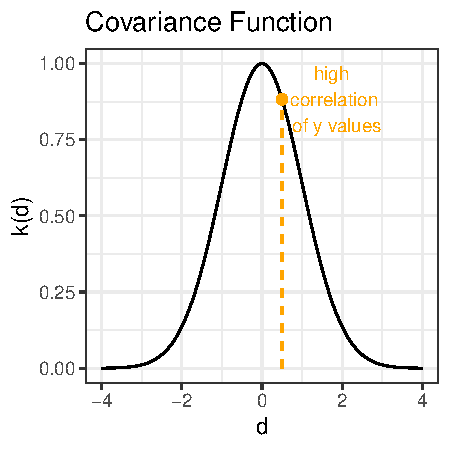
\includegraphics[width=0.45\textwidth]{figure/covariance2point/example_covariance_1.pdf}
%       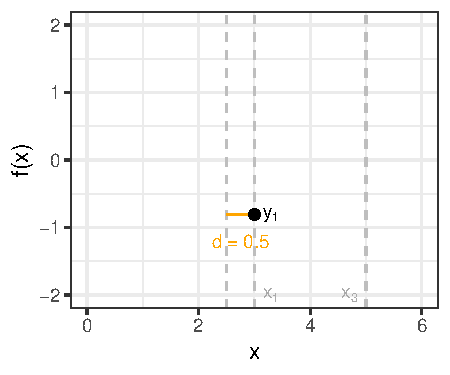
\includegraphics[width=0.45\textwidth]{figure/covariance2point/example_function_1_1.pdf}
%     \end{figure}
% \end{itemize}

% \end{frame}

% \begin{vbframe}{Covariance Function of a GP: Example} 

% \begin{itemize}
%   \item Assume we observed a value $\yi[1] = - 0.8$, the value of $\yi[2]$ should be close under the assumption of the above Gaussian process. 
% \end{itemize}

% \begin{figure}
%   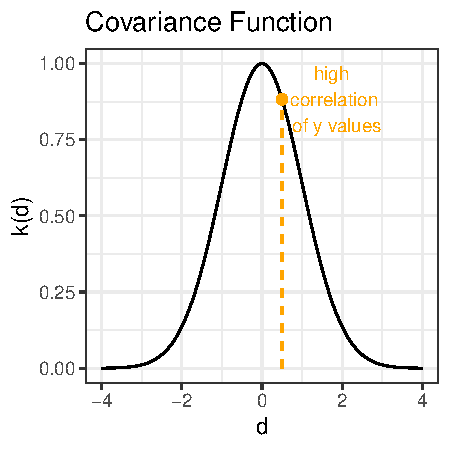
\includegraphics[width=0.45\textwidth]{figure/covariance2point/example_covariance_1.pdf} ~      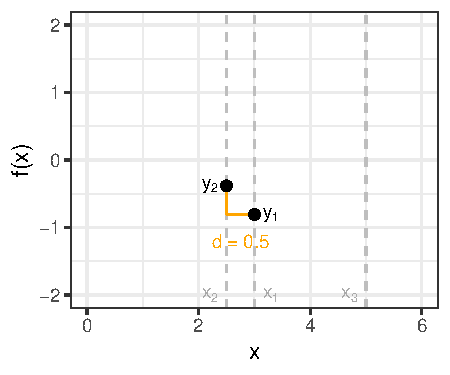
\includegraphics[width=0.45\textwidth]{figure/covariance2point/example_function_1_2.pdf}
% \end{figure}

% \end{vbframe}


% \begin{vbframe}{Covariance Function of a GP: Example} 

% \begin{itemize}
%   \item Let us compare another point $\xi[3]$ to the point $\xi[1]$
%   \item We again compute their correlation
%   \item Their function values are not very much correlated; $\yi[1]$ and $\yi[3]$ might be far away from each other
% \end{itemize}

% \begin{figure}
%   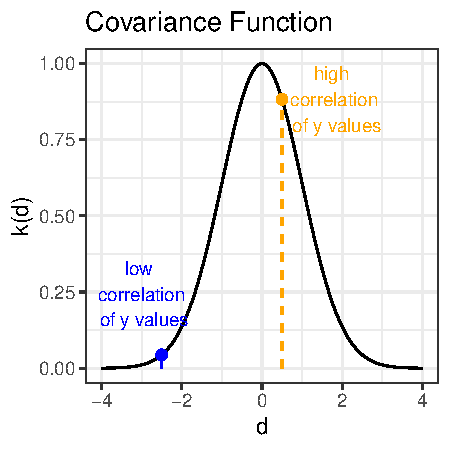
\includegraphics[width=0.45\textwidth]{figure/covariance2point/example_covariance_2.pdf} ~      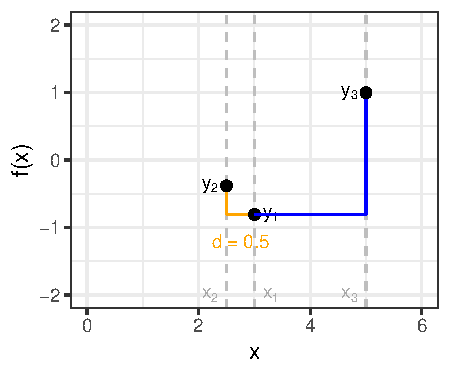
\includegraphics[width=0.45\textwidth]{figure/covariance2point/example_function_2_1.pdf}
% \end{figure}

% \end{vbframe}

% Given an initial point $\xv^{(1)} = 3$ with $f(\xv^{(1)}) = -0.8$, we want to draw a function value for $\xv^{(2)} = 2.5$. 

% \begin{center}
% \includegraphics{figure_man/covariance2point_1.png}
% \end{center}
% }

% \only<2>{Calculating the distance and using the kernel function as a \enquote{look-up-table} for the correlation of the function values, we see that they are highly correlated. We expect the $y$ values being close.  }

% \only<2>{
% \begin{center}
% \includegraphics{figure_man/covariance2point_2.png}
% \end{center}}

% \only<3->{If in comparison we want to draw a function value for at $x^{(3)} = 5$ given $x^{(1)}$ we see on the right plot that the correlation is low. We do not expect the function value being close to $y^{(1)}$. }

% \only<3>{
% \begin{center}
% \includegraphics{figure_man/covariance2point_3.png}
% \end{center}}

% \only<4>{
% \begin{center}
% \includegraphics{figure_man/covariance2point_4.png}
% \end{center}}



% \begin{vbframe}{Covariance Functions}

% There are three types of commonly used covariance functions:

% \begin{itemize}

% \item $k(.,.)$ is called stationary if it is as a function of $\bm{d} = \bm{x} - \bm{x}^\prime$, we write $k(\bm{d})$.\\
% Stationarity is invariance to translations in the input space: $k(\bm{x},\bm{x} + \bm{d}) = k(\bm{0}, \bm{d})$
% \item $k(.,.)$ is called isotropic if it is a function of $r = \|\bm{x} - \bm{x}^\prime\|$, we write $k(r)$.\\
% Isotropy is invariance to rotations of the input space and implies stationarity. 
% \item $k(., .)$ is a dot product covariance function if $k$ is a function of $\bm{x}^T \bm{x}^\prime$
% \end{itemize}

% \end{vbframe}


% \begin{vbframe}{Commonly used covariance functions}
% \textcolor{red}{raus - cheatsheet}
% \begin{table}[]
% \centering
% \begin{tabular}{|c|c|}
% \hline
% Name & $k(\bm{x}, \bm{x}^\prime)$\\
% \hline
% constant & $\sigma_0^2$ \\ [1em]
% linear & $\sigma_0^2 + \bm{x}^T\bm{x}^\prime$ \\ [1em]
% polynomial & $(\sigma_0^2 + \bm{x}^T\bm{x}^\prime)^p$ \\ [1em]
% squared exponential & $\exp(- \frac{\|\bm{x} - \bm{x}^\prime\|^2}{2\ls^2})$ \\ [1em]
% Matérn & \begin{footnotesize} $\frac{1}{2^\nu \Gamma(\nu)}\biggl(\frac{\sqrt{2 \nu}}{\ls}\|\bm{x} - \bm{x}^\prime\|\biggr)^{\nu} K_\nu\biggl(\frac{\sqrt{2 \nu}}{\ls}\|\bm{x} - \bm{x}^\prime\|\biggr)$\end{footnotesize}  \\ [1em]
% exponential & $\exp\left(- \frac{\|\bm{x} - \bm{x}^\prime\|}{\ls}\right)$ \\ [1em]
% \hline
% \end{tabular}
% \end{table}
% \begin{footnotesize}
% $K_\nu(\cdot)$ is the modified Bessel function of the second kind.
% \end{footnotesize}


% \begin{center}

% \includegraphics{figure/covariance.pdf}
% \end{center}
% \vskip -1 em
% \begin{footnotesize}
% \begin{itemize}
% \item Random functions drawn from Gaussian processes with a Squared Exponential Kernel (left), Polynomial Kernel (middle), and a Matérn Kernel (right, $\ls = 1$). 
% \item The length-scale hyperparameter determines the ``wiggliness'' of the function.
% \item For Matérn, the $\nu$ parameter determines how differentiable the process is.
% \end{itemize}
% \end{footnotesize}
% \end{vbframe}

% \begin{vbframe}{Making New Kernels from Old}

% Kernels can be

% \begin{itemize}
% \item Summed together
% \begin{itemize}
% \item on the same space $k(\xv, \xv') = k_1(\xv, \xv') + k_2(\xv, \xv')$
% \item on tensor space $k(\xv, \xv') = k_1(x_1, x_1') + k_2(x_2, x_2')$
% \end{itemize}
% \item Multiplied together
% \begin{itemize}
% \item on the same space $k(\xv, \xv') = k_1(\xv, \xv') \cdot k_2(\xv, \xv')$
% \item on tensor space $k(\xv, \xv') = k_1(x_1, x_1') \cdot k_2(x_2, x_2')$
% \end{itemize}
% \item Composed with a function $k(\xv, \xv') = k_1(g(\xv), g(\xv'))$ 
% \end{itemize}

% All these operations will preserve the positive definiteness (see exercise). 
% More details: lecture about kernel methods.

% \end{vbframe}
%-----------------------------------------------------------------------

% \begin{vbframe}{Squared Exponential Covariance Function}

% The squared exponential function is one of the most commonly used covariance functions.
% $$
% k(\xv, \tilde{\xv}) = \exp\biggl(- \frac{\|\xv - \tilde{\xv}\|^2}{2\ls^2}\biggr).
% $$

% \textbf{Properties}:
% \begin{itemize}
% \item It depends merely on the distance $r = \|\xv - \tilde{\xv}\|$ $\to$ isotropic and stationary.\lz
% \item Infinitely differentiable $\to$ sometimes deemed 
%   unrealistic for modeling most of the physical processes.

% \end{itemize}

% \end{vbframe}

%%%%%%%%%%%%%%%%%%%%%%%%%%%%%%%%%%%%%%%%%%%%%%%%%%%%%%%%%%%%%%%%%%%%%%%%%%%%%%%%%%%%
% \begin{frame}[c,allowframebreaks]{Characteristic Length-Scale}
    % $$k(\xv, \tilde{\xv}) = \exp\left(-\frac{1}{2\ls^2}\|\xv - \tilde{\xv}\|^2\right)$$
% \begin{figure}
	% \includegraphics[width = .8\textwidth]{figure/lengthscale-1.pdf}
% \end{figure}
% $\ls$ is called \textbf{characteristic length-scale}. Loosely speaking, the characteristic length-scale describes how far you need to move in input space for the function values to become uncorrelated. Higher $\ls$ induces smoother functions, lower $\ls$ induces more wiggly functions.

% \begin{figure}
% \includegraphics[width=0.6\textwidth]{figure/gp_sample/varying_length_scale.pdf}
% \end{figure}

% \begin{itemize}
    % \item Left: for higher $\ls$ the correlation between function values (for unchanged distance of input points) is also higher
    % \item Right plot: a higher $\ls$ induces a smoother function 
% \end{itemize}

% \framebreak

% For $p \geq 2$ dimensions, the squared exponential can be parameterized:

% $$
% k(\xv, \tilde{\xv}) = \exp\,\biggl(- \frac{1}{2}\left(\xv - \tilde{\xv}\right)^\top\bm{M}\left(\xv - \tilde{\xv} \right)\biggr)
% $$

% Possible choices for the matrix $\bm{M}$ include

% $$
% \bm{M}_1 = \ls^{-2}\id \qquad \bm{M}_2 = \text{diag}(\bm{\ls})^{-2} \qquad \bm{M}_3 = \Gamma \Gamma^\top + \text{diag}(\bm{\ls})^{-2}
% $$

% where $\bm{\ls}$ is a $p$-vector of positive values and $\Gamma$ is a $p \times k$ matrix. 

% \lz

% The 2nd (and most important) case can also be written as 
% $$
%   k(\bm{d}) = \exp\,\biggl(- \frac{1}{2} \sumjp \frac{d_j^2}{l_j^2} \biggr)
% $$

% Here again, $\bm{\ls} = (\ls_1,\dots, \ls_p)$ are characteristic length-scales for each dimension. 


% \framebreak


% What is the benefit of having an individual hyperparameter $\ls_i$ for each dimension?

% \vspace{4mm}

% \begin{itemize} 
% \item The $\ls_1,\dots, \ls_p$ hyperparameters play the role of \textbf{characteristic length-scales}.
% \vspace{2mm}
% \item Loosely speaking, $\ls_i$ describes how far you need to move along axis $i$ in input space for the function values to be uncorrelated.
% \vspace{2mm}
% \item Such a covariance function implements \textbf{automatic relevance determination} (ARD), since the inverse of the length-scale $\ls_i$ determines the relevancy of input feature $i$ to the regression.
% \vspace{2mm}
% \item If $\ls_i$ is very large, the covariance will become almost independent of that input, effectively removing it from inference.
% \vspace{2mm}
% \item If the features are on different scales, the data can be automatically \textbf{rescaled} by estimating $\ls_1,\dots, \ls_p$ 

% \end{itemize}



% \framebreak


% \begin{figure}
% 	\includegraphics[width = .8\textwidth]{figure_man/covariance2D.png}
% \end{figure}

% \vspace{3mm}
% %\begin{footnotesize}
% For the first plot, we have chosen $\bm{M} = \id$: the function varies the same in all directions. The second plot is for $\bm{M} = \text{diag}(\bm{\ls})^{-2}$ and $\bm{\ls} = \left(1, 3 \right)$: The function varies less rapidly as a function of $x_2$ than $x_1$ as the length-scale for $x_1$ is less. In the third plot $\bm{M} = \Gamma \Gamma^T + \text{diag}(\bm{\ls})^{-2}$ for $\Gamma = (1, -1)^\top$ and $\bm{\ls} = (6, 6)^\top$. Here $\Gamma$ gives the direction of the most rapid variation. (Image from Rasmussen \& Williams, 2006)
% %\end{footnotesize}


% \end{frame}

\endlecture
\end{document}

